\section{Date: 2026-08-27}
\noindent \textbf{Series ID: CIU2013000100000I} 

\noindent This series is titled Employment Cost Index: Total compensation for Private industry workers in Manufacturing; management, professional, and related occupations and has a frequency of Quarterly. The units are Index Dec 2005=100 and the seasonal adjustment is Not Seasonally Adjusted.The observation start date is 2001-01-01 and the observation end date is 2026-04-01.The popularity of this series is 3. \\ 

\noindent \textbf{Series ID: CWSR0000SAF11} 

\noindent This series is titled Consumer Price Index for All Urban Wage Earners and Clerical Workers: Food at Home in U.S. City Average and has a frequency of Monthly. The units are Index 1982-1984=100 and the seasonal adjustment is Seasonally Adjusted.The observation start date is 1952-01-01 and the observation end date is 2026-07-01.The popularity of this series is 1. \\ 

\subsection{Raw Regression}
\noindent Regresses the two series against each other directly. A significant result here can come just as easily from both series sharing a long-run trend as from any real relationship.

\begin{center}
\begin{tabular}{lclc}
\toprule
\textbf{Dep. Variable:}                 & value\_fred\_CWSR0000SAF11 & \textbf{  R-squared:         } &     0.952   \\
\textbf{Model:}                         &            OLS             & \textbf{  Adj. R-squared:    } &     0.951   \\
\textbf{Method:}                        &       Least Squares        & \textbf{  F-statistic:       } &     1958.   \\
\textbf{Date:}                          &      Thu, 27 Aug 2026      & \textbf{  Prob (F-statistic):} &  4.92e-67   \\
\textbf{Time:}                          &          21:22:56          & \textbf{  Log-Likelihood:    } &   -363.32   \\
\textbf{No. Observations:}              &              101           & \textbf{  AIC:               } &     730.6   \\
\textbf{Df Residuals:}                  &               99           & \textbf{  BIC:               } &     735.9   \\
\textbf{Df Model:}                      &                1           & \textbf{                     } &             \\
\textbf{Covariance Type:}               &         nonrobust          & \textbf{                     } &             \\
\bottomrule
\end{tabular}
\begin{tabular}{lcccccc}
                                        & \textbf{coef} & \textbf{std err} & \textbf{t} & \textbf{P$> |$t$|$} & \textbf{[0.025} & \textbf{0.975]}  \\
\midrule
\textbf{const}                          &      10.1646  &        5.080     &     2.001  &         0.048        &        0.085    &       20.245     \\
\textbf{value\_fred\_CIU2013000100000I} &       1.8620  &        0.042     &    44.250  &         0.000        &        1.779    &        1.946     \\
\bottomrule
\end{tabular}
\begin{tabular}{lclc}
\textbf{Omnibus:}       &  5.948 & \textbf{  Durbin-Watson:     } &    0.072  \\
\textbf{Prob(Omnibus):} &  0.051 & \textbf{  Jarque-Bera (JB):  } &    5.044  \\
\textbf{Skew:}          & -0.455 & \textbf{  Prob(JB):          } &   0.0803  \\
\textbf{Kurtosis:}      &  2.391 & \textbf{  Cond. No.          } &     691.  \\
\bottomrule
\end{tabular}
%\caption{OLS Regression Results}
\end{center}

Notes: \newline
 [1] Standard Errors assume that the covariance matrix of the errors is correctly specified.

\begin{figure}
\centering
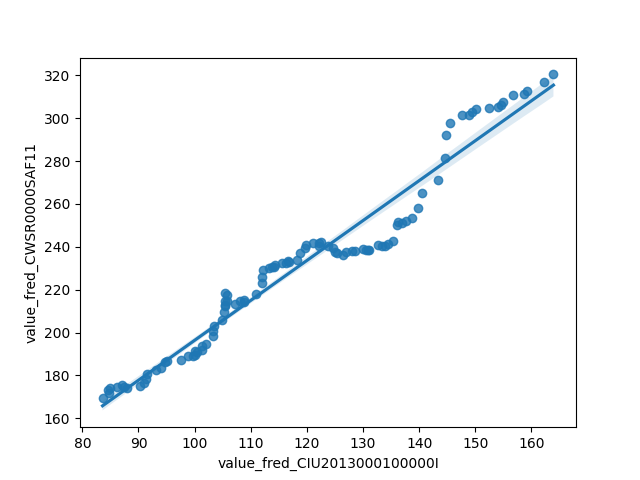
\includegraphics[scale = 0.9]{plots/plot_2026-08-27.png}
\caption{Raw Regression Plot for 2026-08-27}
\end{figure}
\newpage
\subsection{Detrended Regression}
\noindent Regresses the residuals of each series after removing its own linear time trend, so a shared trend can no longer drive the result on its own. A relationship that stays significant here is better evidence of a genuine link between the two series.

\begin{center}
\begin{tabular}{lclc}
\toprule
\textbf{Dep. Variable:}                            & value\_fred\_CWSR0000SAF11\_detrended & \textbf{  R-squared:         } &     0.434   \\
\textbf{Model:}                                    &                  OLS                  & \textbf{  Adj. R-squared:    } &     0.428   \\
\textbf{Method:}                                   &             Least Squares             & \textbf{  F-statistic:       } &     75.78   \\
\textbf{Date:}                                     &            Thu, 27 Aug 2026           & \textbf{  Prob (F-statistic):} &  7.23e-14   \\
\textbf{Time:}                                     &                21:22:57               & \textbf{  Log-Likelihood:    } &   -358.47   \\
\textbf{No. Observations:}                         &                    101                & \textbf{  AIC:               } &     720.9   \\
\textbf{Df Residuals:}                             &                     99                & \textbf{  BIC:               } &     726.2   \\
\textbf{Df Model:}                                 &                      1                & \textbf{                     } &             \\
\textbf{Covariance Type:}                          &               nonrobust               & \textbf{                     } &             \\
\bottomrule
\end{tabular}
\begin{tabular}{lcccccc}
                                                   & \textbf{coef} & \textbf{std err} & \textbf{t} & \textbf{P$> |$t$|$} & \textbf{[0.025} & \textbf{0.975]}  \\
\midrule
\textbf{const}                                     &   -1.722e-12  &        0.846     & -2.04e-12  &         1.000        &       -1.679    &        1.679     \\
\textbf{value\_fred\_CIU2013000100000I\_detrended} &       2.9108  &        0.334     &     8.705  &         0.000        &        2.247    &        3.574     \\
\bottomrule
\end{tabular}
\begin{tabular}{lclc}
\textbf{Omnibus:}       & 16.748 & \textbf{  Durbin-Watson:     } &    0.103  \\
\textbf{Prob(Omnibus):} &  0.000 & \textbf{  Jarque-Bera (JB):  } &    4.910  \\
\textbf{Skew:}          & -0.158 & \textbf{  Prob(JB):          } &   0.0859  \\
\textbf{Kurtosis:}      &  1.967 & \textbf{  Cond. No.          } &     2.53  \\
\bottomrule
\end{tabular}
%\caption{OLS Regression Results}
\end{center}

Notes: \newline
 [1] Standard Errors assume that the covariance matrix of the errors is correctly specified.

\begin{figure}
\centering
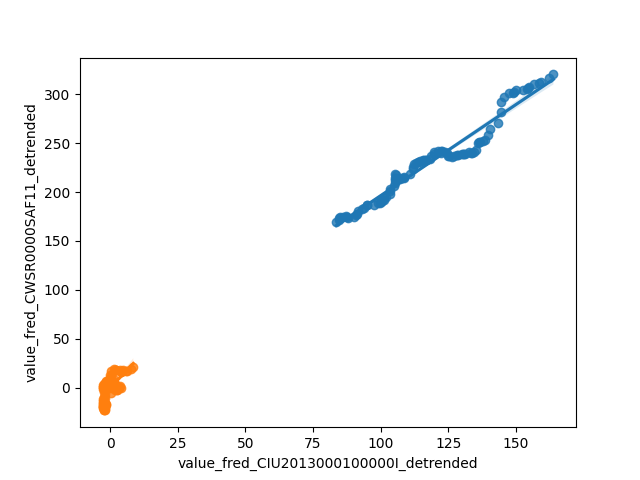
\includegraphics[scale = 0.9]{plots/plot_2026-08-27_detrended.png}
\caption{Detrended Regression Plot for 2026-08-27}
\end{figure}
\newpage
